\documentclass{standalone}
\usepackage{tikz}
\usetikzlibrary{arrows}

\begin{document}

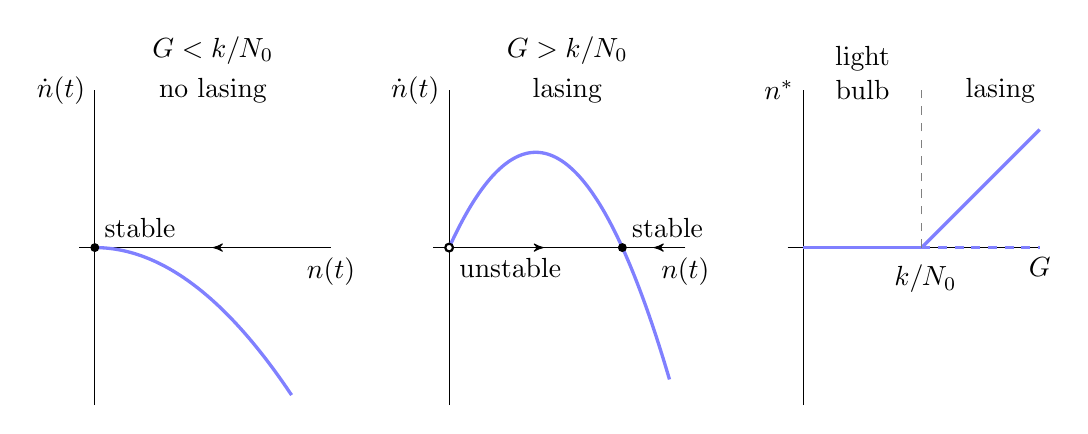
\begin{tikzpicture}
\begin{scope}
  \draw[] (-0.2,0) -- (3,0) node[below] {$n(t)$};
  \draw[] (0,-2) -- (0,2) node[left] {$\dot{n}(t)$};
  \draw[blue!50, variable=\x, samples at={0,0.01,...,2.5}, very thick] plot (\x,{-0.3*\x*\x});
  \filldraw[black, draw=black] (0,0) circle (1.4pt) node[above right] {stable};
  \draw[-stealth'] (2,0) -- (1.5,0);
  \node[] at (1.5,2.5) {$G<k/N_0$};
  \node[] at (1.5,2) {no lasing};
\end{scope}

\begin{scope}[xshift=4.5cm]
  \draw[] (-0.2,0) -- (3,0) node[below] {$n(t)$};
  \draw[] (0,-2) -- (0,2) node[left] {$\dot{n}(t)$};
  \draw[blue!50, variable=\x, samples at={0,0.01,...,2.8}, very thick] plot (\x,{2.2*\x-\x*\x});
  \filldraw[white, draw=black, thick] (0,0) circle (1.4pt) node[below right, black] {unstable};
  \filldraw[black, draw=black] (2.2,0) circle (1.4pt) node[above right] {stable};
  \draw[-stealth'] (1,0) -- (1.2,0);
  \draw[-stealth'] (3,0) -- (2.6,0);
  \node[] at (1.5,2.5) {$G>k/N_0$};
  \node[] at (1.5,2) {lasing};
\end{scope}

\begin{scope}[xshift=9cm]
  \draw[] (-0.2,0) -- (3,0) node[below] {$G$};
  \draw[] (0,-2) -- (0,2) node[left] {$n^*$};
  \draw[blue!50, variable=\x, samples at={0,0.01,...,1.5}, very thick] plot (\x,0);
  \draw[blue!50, variable=\x, samples at={1.5,1.51,...,3}, very thick, dashed] plot (\x,0);
  \draw[blue!50, variable=\x, samples at={1.5,1.51,...,3}, very thick] plot (\x,\x-1.5);
  \draw[black!50, dashed] (1.5,0) -- (1.5,2);
  \node[] at (1.55,-0.4) {$k/N_0$};
  \node[] at (0.75,2.4) {light};
  \node[] at (0.75,2) {bulb};
  \node[] at (2.5,2) {lasing};
\end{scope}
  
\end{tikzpicture}

\end{document}